\documentclass[a4paper,12pt]{article}    % Specifies the document style.

\usepackage[top=2cm, bottom=2cm]{geometry}

\usepackage{amsfonts}

\usepackage[utf8]{inputenc} % Permite o uso de acentos sem precisar de escapes (\', \~ etc)
\usepackage[brazilian]{babel} % Hifenização em português, datas, seções etc em português

\usepackage{graphicx}
\usepackage{caption}
\usepackage{subcaption}
\usepackage{url}

\usepackage{listings} % colocar código
\lstset{ %
language=XML,                % choose the language of the code
breaklines=true,                % sets automatic line breaking
breakatwhitespace=true,        % sets if automatic breaks should only happen at whitespace
}

\usepackage[usenames]{color}

% keywords
\newcommand{\keywords}[1]{\par\noindent
{\small{\bf Palavras-chave\/}: #1}}

\newcommand{\degree}{\ensuremath{^\circ}}

\title{Relatório de Iniciação Científica \\
Técnicas Espectrais para Agrupamento Múltiplo}
\author{Mateus Matias dos Santos, aluno \\
Eduardo Bezerra da Silva, orientador}
\date{Agosto de 2015}

\begin{document}

\begin{titlepage}
\maketitle
\end{titlepage}

\begin{abstract}
Este projeto de pesquisa visa o aprofundamento em técnicas espectrais de redução de dimensionalidade, especificamente a baseada em autovetores e autovalores\footnote{\textit{eigenvectors e eigenvalues.}}, com o objetivo de facilitar o agrupamento de conjuntos de dados (\textit{datasets}) que possuem uma distribuição reminiscente da distribuição normal ou Gaussiana, ou tantas dimensões que cause inconsistências no resultado de algoritmos de agrupamento. Essa técnica, no contexto desse projeto, é usada para tratamento de dados astronômicos correspondentes à estrelas, possibilitando o agrupamento de sistemas estelares que possuem a mesma origem (um \textit{open cluster}). A linguagem de programação utilizada é o Python versão 3.3.

\keywords{grafo, distribuição normal, eigenvectors, clustering, estrelas, \textit{open cluster}}
\end{abstract}
\newpage

\tableofcontents
\newpage

\section{Introdução}

A redução de dimensionalidade é de vital importância ao lidar com datasets dispostos de forma normal e com muitas dimensões, pois facilita a comparação e, consequentemente, a aplicação de algoritmos de agrupamento, já que se estes baseiam principalmente em estabelecer uma relação entre os dados. Uma das áreas em que é necessária a redução de dimensionalidade de datasets é na Astronomia. Entre os diversos problemas que requerem o auxílio da computação, destaco o \textit{Stellar Cluster Membership Assignment}, definido como ``o problema de segregar o campo e estrelas que pertencem a um mesmo aglomerado em um dado campo de catálogos que são gerados a partir de imagens de um telescópio''[1]. Os dados de entrada são as coordenadas $x$ e $y$ de cada estrela; o $z$, porém, não é conhecido, o que impossibilita o uso de algoritmos de agrupamento tradicionais. Por isso, é necessária a redução de dimensionalidade do dataset, para que se possa aplicar tais técnicas. O método de redução de dimensionalidade usado é aquele segundo Belkin e Niyogi[2], valendo-se de \textit{eigenmaps} e técnicas espectrais para clustering, aplicado a um dataset bi-dimensional gerado aleatoriamente nos padrões dos dados destacados anteriormente.

\section{Desenvolvimento}

\subsection{Funções}

A base da implementação consiste em três funções:

\begin{itemize}
	\item[(i)] \textit{create\_dataset(N, cov1, cov2, mean1=[1,1], mean2=[1,1])}, onde $N$ é o número de elementos, $cov1$ é a matriz de covariância que gera o primeiro agrupamento; $cov2$ é a matriz de covariância que gera o segundo agrupamento; $mean1$ indica a posição $x$ e $y$ do ponto médio do primeiro agrupamento e $mean2$ indica a posição $x$ e $y$ do ponto médio do segundo agrupamento. O retorno dessa função é uma matriz $R^{N \times 3}$ que contém os valores $x$ e $y$ de cada objeto e uma coluna destinada a informar a qual cluster o objeto pertence. O objetivo dessa função é gerar um dataset que consista em dois agrupamentos gerados através da distribuição normal multivariada e depois plotá-lo na tela. As bibliotecas utilizadas são: 
	\begin{itemize}
		\item[(i.i)] numpy, que conta com inúmeras funcionalidades matemáticas prontas. Nesse caso, foi utilizada a função \textit{numpy.random.multivariate\_normal(mean1, cov1, N)}, que recebe como parâmetro um ponto central, uma matriz de covariância e um número de elementos e gera um dataset aleatório seguindo o padrão multivariado normal; e
		\item[(i.ii)] matplotlib, usado para plotar\footnote{Desenhar} o dataset gerado em um gráfico.
	\end{itemize}
	\item[(ii)] \textit{en\_heat(n\_samples, ep, t, D)}, onde $n\_samples$ é o número de elementos presentes no \textit{dataset}, $ep$ (epsilon) e $t$ são paramêtros oriundos da escolha pelos métodos \textit{$e$-neighborhoods} e \textit{heat kernel}[2], e $D$ é a matriz dos dados aos quais será aplicada a redução dimensional. O objetivo dessa função é implementar as técnicas de redução de dimensionalidade descritas por Belkin e Niyogi[2] e plotar o resultado. As bibliotecas utilizadas são:
		\begin{itemize}
			\item[(ii.i)] numpy, pela função numpy.linalg.eig(R), que retorna os eigenvalues e eigenvectors de uma matriz R;
			\item[(ii.ii)] matplotlib, usado para plotar o dataset reduzido em um gráfico; e
			\item[(ii.iii)] scikit-learn, abreviado sklearn, que possui funções relacionadas ao aprendizado de máquina. Nessa função, foi chamada a função \textit{sklearn.preprocessing.normalize} com o propósito de normalizar os dados do dataset de entrada.
		\end{itemize}
	\item[(iii)] \textit{pca\_plot(X, n\_samples)}, onde X é a matriz a qual será aplicada o PCA e $n\_samples$ é o número de elementos presentes no \textit{dataset}. É uma implementação simples que reduz a dimensionalidade do dataset para 1 e plota o resultado. As bibliotecas utilizadas são:
		\begin{itemize}
			\item[(iii.i)] numpy;
			\item[(iii.ii)] matplotlib; e
			\item[(iii.iii)] sklearn, pela função \textit{sklearn.decomposition.PCA}, uma implementação do algoritmo PCA.
		\end{itemize}
\end{itemize}

\newpage
\subsection{Comparações com PCA}

Nessa seção serão mostrados resultados comparativos de cinco datasets gerados pela função \textit{create\_dataset}, nos quais foram aplicadas as funções \textit{en\_heat} e \textit{pca\_plot}.

\subsubsection{Dataset 1}
\begin{figure}[!hb]
	\centering
	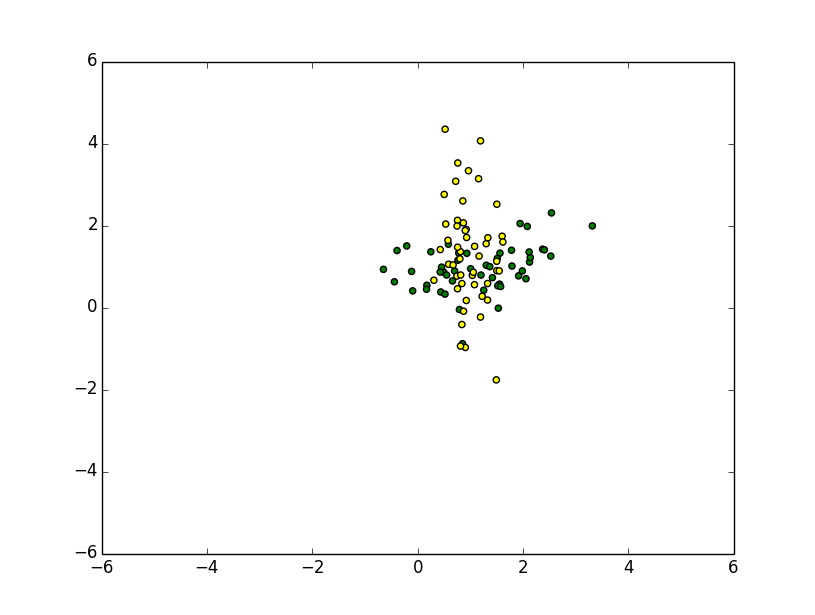
\includegraphics[width=\linewidth]{img/1dataset.png}
	\caption*{N=100, cov1=[[0.1, 0], [0, 2]], cov2=[[0.9, 0.2], [0.2, 0.3]]}
	\begin{subfigure}{.45\textwidth}
		\centering
		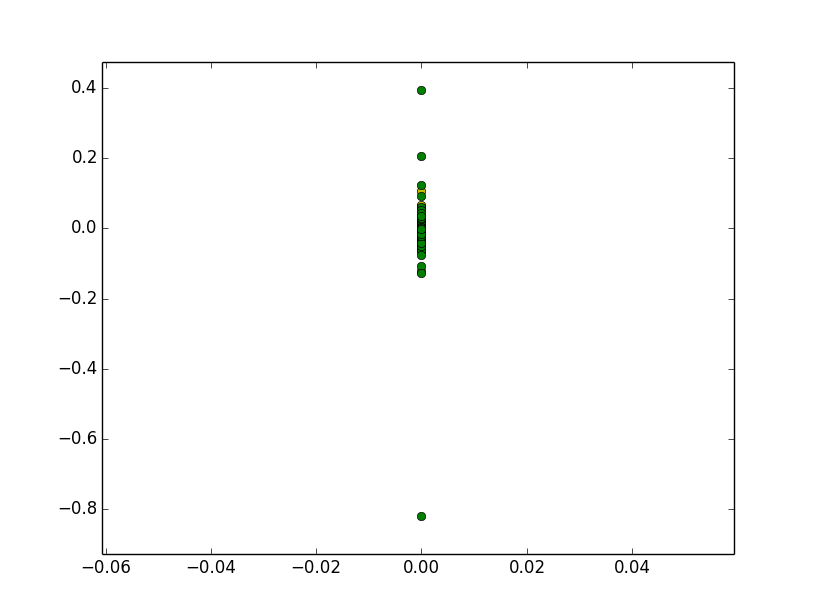
\includegraphics[width=\linewidth]{img/2spectral.png}
		\caption{Método Espectral}
	\end{subfigure}
	\begin{subfigure}{.45\textwidth}
		\centering
		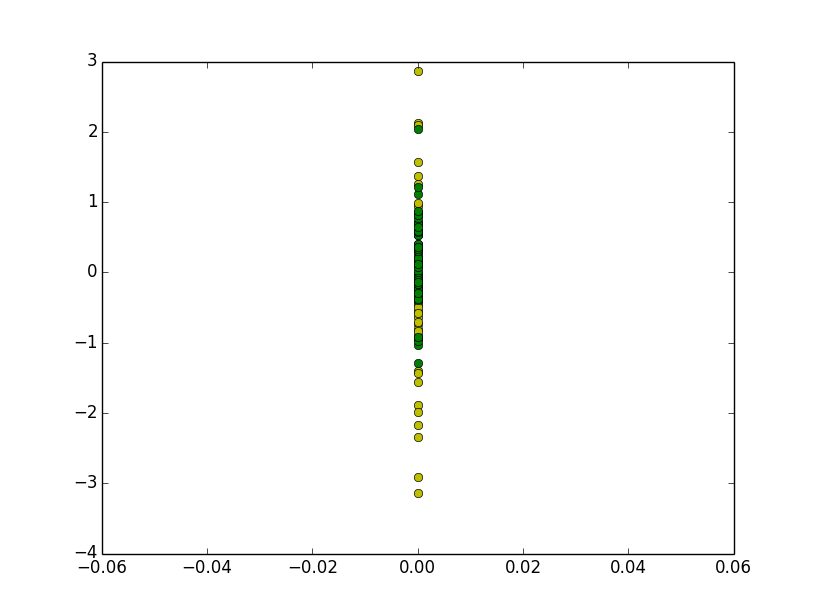
\includegraphics[width=\linewidth]{img/3pca.png}
		\caption{PCA}
	\end{subfigure}
	\label{dataset1}
\end{figure}
\vfill
\clearpage

\subsubsection{Dataset 2}
\begin{figure}[!ht]
	\centering
	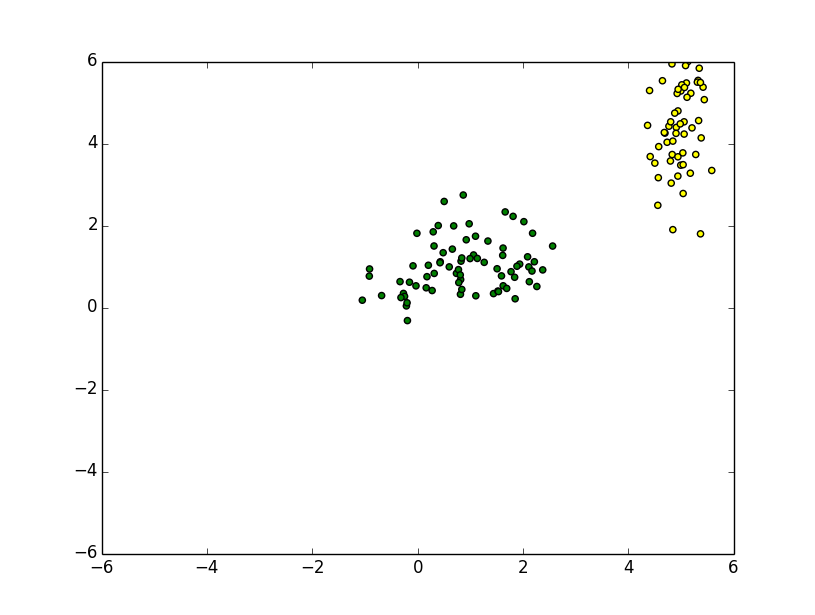
\includegraphics[width=\linewidth]{img/4dataset.png}
	\caption*{N=150, cov1=[[0.1, 1], [0, 2]], cov2=[[0.9, 0.2], [0.2, 0.3]], mean1=[5, 5]}
	\begin{subfigure}{.45\textwidth}
		\centering
		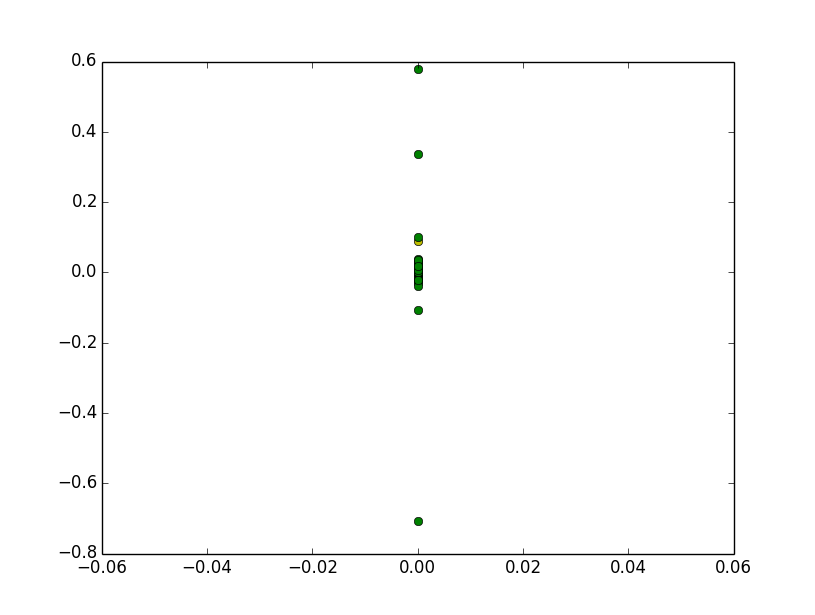
\includegraphics[width=\linewidth]{img/5spectral.png}
		\caption{Método Espectral}
	\end{subfigure}
	\begin{subfigure}{.45\textwidth}
		\centering
		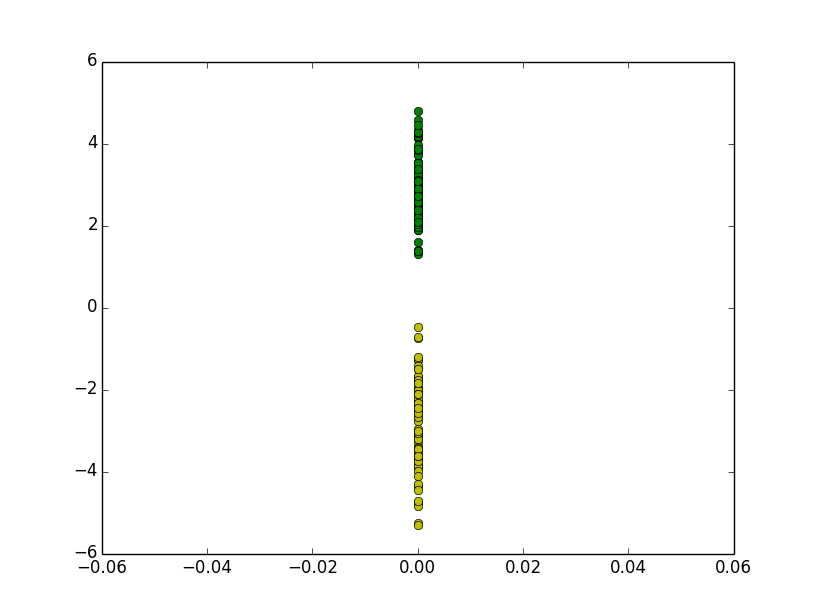
\includegraphics[width=\linewidth]{img/6pca.png}
		\caption{PCA}
	\end{subfigure}
	\label{dataset2}
\end{figure}
\vfill
\clearpage

\subsubsection{Dataset 3}
\begin{figure}[!ht]
	\centering
	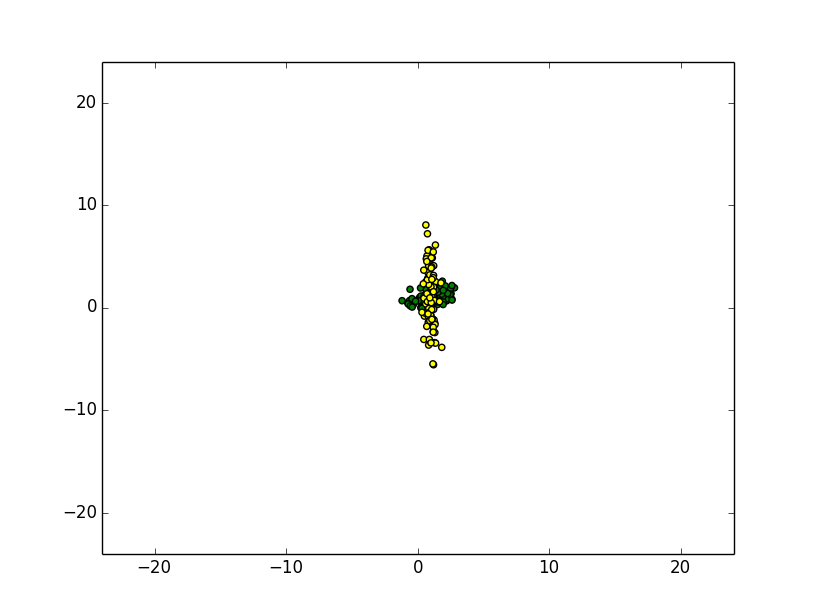
\includegraphics[width=\linewidth]{img/7dataset.png}
	\caption*{N=200, cov1=[[0.1, 0], [0, 8]], cov2=[[0.9, 0.2], [0.2, 0.3]]}
	\begin{subfigure}{.45\textwidth}
		\centering
		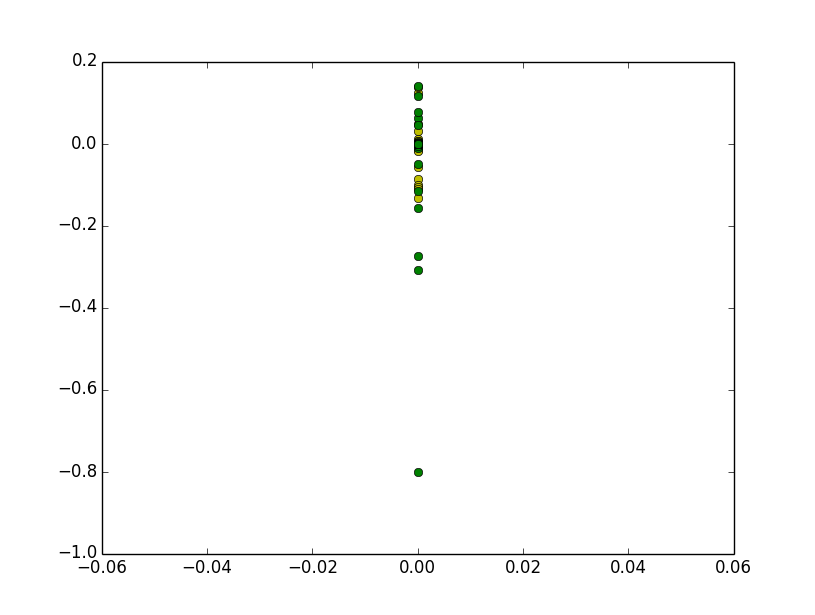
\includegraphics[width=\linewidth]{img/8spectral.png}
		\caption{Método Espectral}
	\end{subfigure}
	\begin{subfigure}{.45\textwidth}
		\centering
		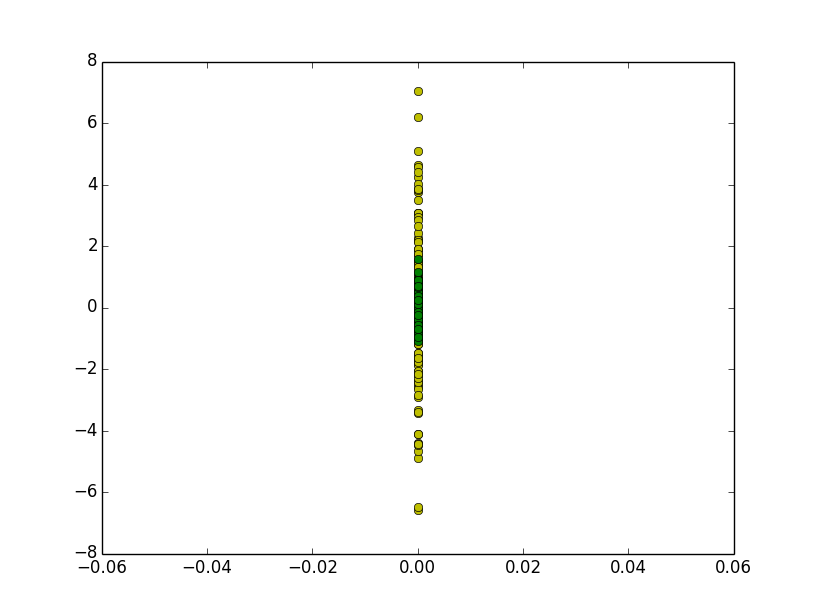
\includegraphics[width=\linewidth]{img/9pca.png}
		\caption{PCA}
	\end{subfigure}
	\label{dataset3}
\end{figure}
\vfill
\clearpage

\subsubsection{Dataset 4}
\begin{figure}[!ht]
	\centering
	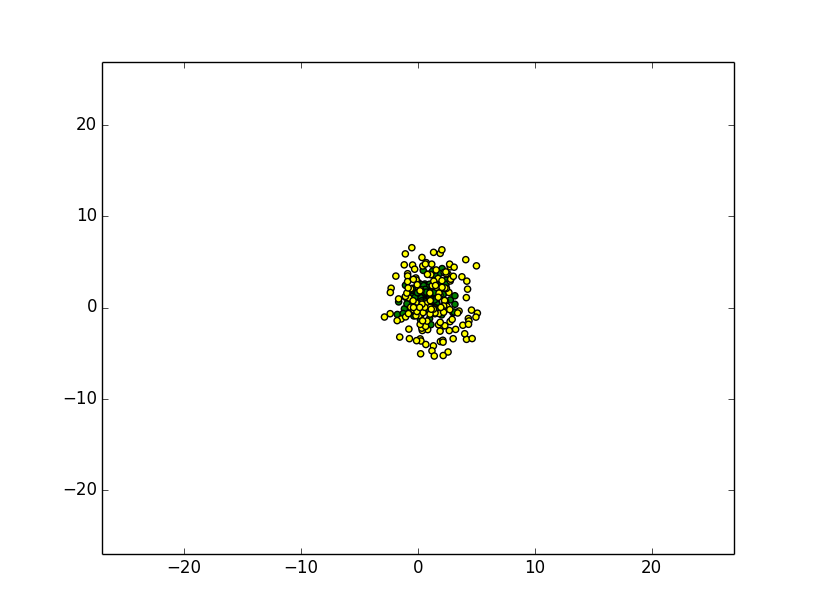
\includegraphics[width=\linewidth]{img/10dataset.png}
	\caption*{N=300, cov1=[[3, 0], [0, 9]], cov2=[[1, 0.2], [0.2, 2.1]]}
	\begin{subfigure}{.45\textwidth}
		\centering
		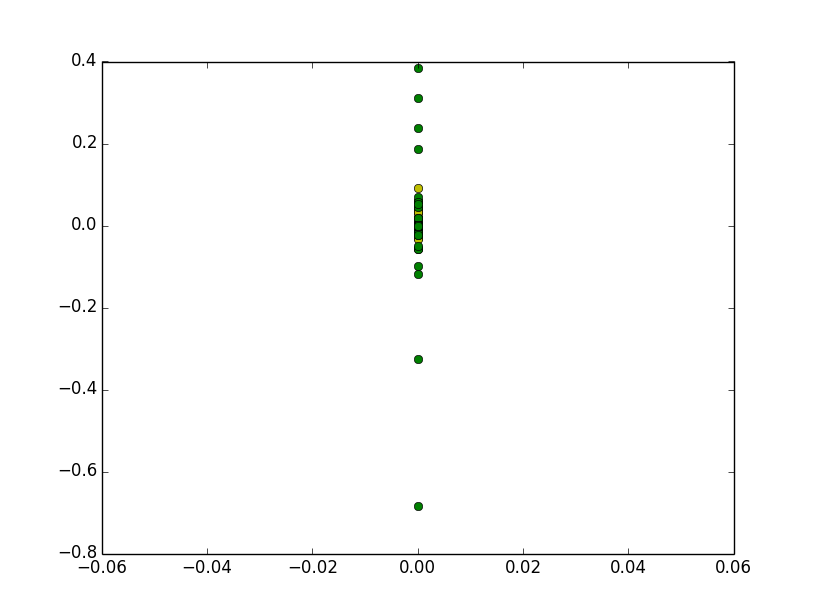
\includegraphics[width=\linewidth]{img/11spectral.png}
		\caption{Método Espectral}
	\end{subfigure}
	\begin{subfigure}{.45\textwidth}
		\centering
		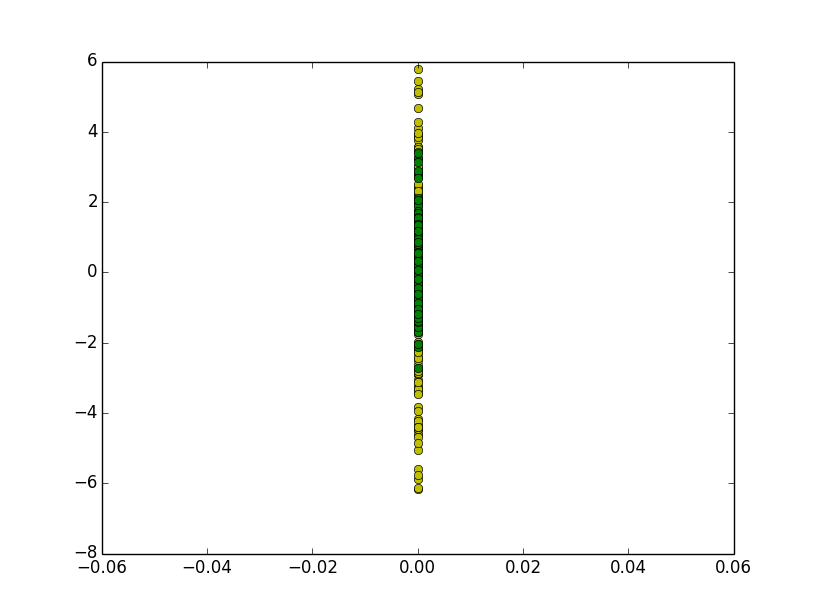
\includegraphics[width=\linewidth]{img/12pca.png}
		\caption{PCA}
	\end{subfigure}
	\label{dataset4}
\end{figure}
\vfill
\clearpage

\subsubsection{Dataset 5}
\begin{figure}[!ht]
	\centering
	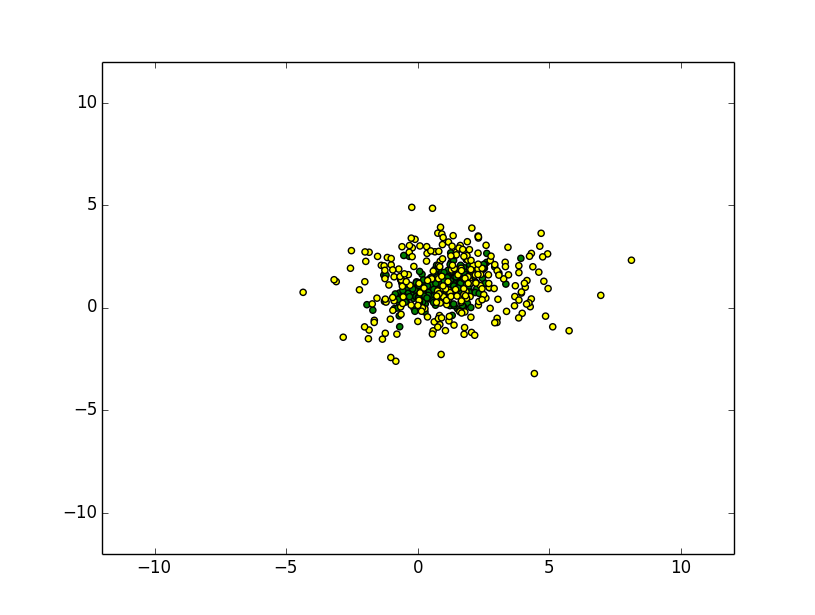
\includegraphics[width=\linewidth]{img/13dataset.png}
	\caption*{N=500, cov1=[[4, 0], [0, 2]], cov2=[[0.9, 0.2], [0.2, 0.3]]}
	\begin{subfigure}{.45\textwidth}
		\centering
		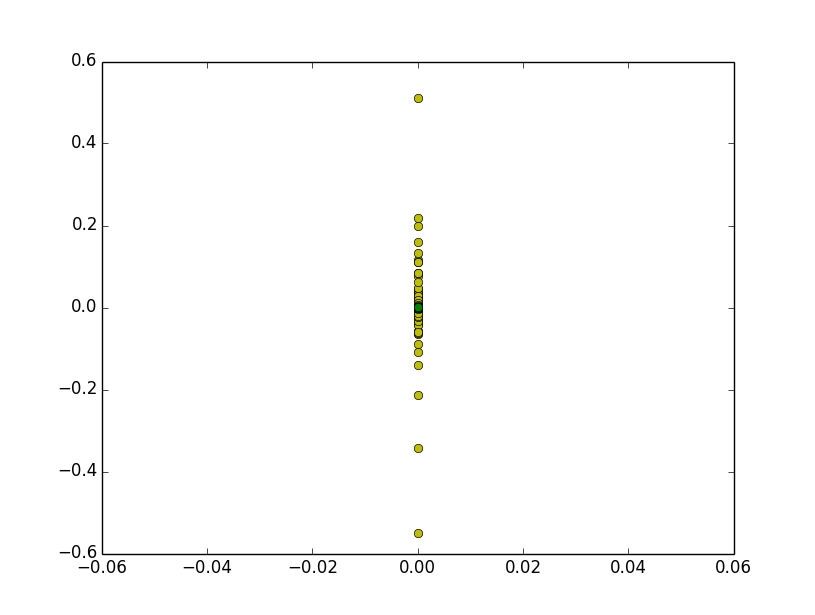
\includegraphics[width=\linewidth]{img/14spectral.png}
		\caption{Método Espectral}
	\end{subfigure}
	\begin{subfigure}{.45\textwidth}
		\centering
		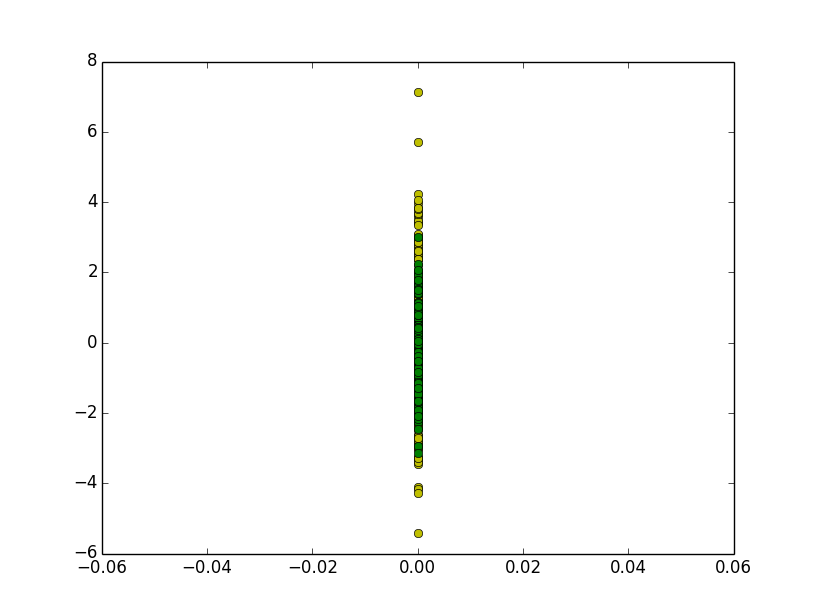
\includegraphics[width=\linewidth]{img/15pca.png}
		\caption{PCA}
	\end{subfigure}
	\label{dataset5}
\end{figure}
\vfill
\clearpage

\section{Conclusão}

Em retrospecto, a experiência de trabalhar com Python foi positiva. Em termos de desenvolvimento, é uma linguagem bem diferente de C, a única que o autor possuía conhecimento, porque conta com uma sintaxe mais simples e bibliotecas específicas voltadas para a área científica.
Houve alguns momentos que o progresso foi afetado por problemas específicos ao lidar com a biblioteca numpy, por esta possuir um tipo específico de \textit{array} (o \emph{ndarray}). Tais obstáculos foram ultrapassados com uma leitura mais profunda sobre o funcionamento da biblioteca. Outros problemas relacionados ao funcionamento da linguagem Python foram resolvidos com pesquisas sobre o tema.
Desse projeto, o autor pôde alcançar um aprendizado básico em álgebra linear, matemática aplicada e Python, que definitivamente serão úteis no futuro.
O autor agradece ao CNPq e ao CEFET/RJ pelo apoio no desenvolvimento desta pesquisa.

\begin{thebibliography}{99}

	\bibitem{BLKM14} Bezerra, E., De Lima, L., Krone-Martins, A. (2014) \emph{Spectral Dimensionality Reduction Applied to Stellar Cluster Membership Assignment}, Many Faces of Distances, Campinas, Brasil.
	
	\bibitem{BN01}
	Belkin, M., Niyogi, P. (2001) \emph{Laplacian Eigenmaps and spectral techniques for embedding and clustering},
	NIPS 14, pp. 585--591, MIT Press.
	
\end{thebibliography}

\end{document}